\documentclass[10pt,a4paper]{article}
\usepackage[utf8]{inputenc}
\usepackage[margin=1in]{geometry}
\thispagestyle{empty}

\usepackage{amsmath}
\usepackage{amsfonts}
\usepackage{amssymb}

\usepackage{parskip}

\usepackage{listings}
\usepackage{xcolor}

\usepackage{enumerate}

\usepackage{hyperref}

\usepackage{float}
\usepackage[font=small,labelfont=bf]{caption}
\usepackage{wrapfig}

\usepackage{graphicx}
\restylefloat{figure}

\usepackage{cancel}

\usepackage{multicol}

\author{Cristian Escudero}
\title{Resumen\\Inteligencia Computacional}
\begin{document}

\section*{Introducción (Unidad I)}
\begin{quote}
Breve revisión histórica a la inteligencia computacional. Áreas del conocimiento involucradas y su relación como parte de la inteligencia artificial. El cerebro humano y las limitaciones del cálculo computacional. El impacto y el amplio espectro de aplicaciones de la inteligencia computacional. Introducción conceptual a las tres técnicas fundamentales de la inteligencia computacional.
\end{quote}

\section*{Redes neuronales 1 (Unidad II)}
\begin{quote}
Bases estadísticas del reconocimiento de patrones: etapas, decisión bayesiana, funciones discriminantes. Aprendizaje, espacio de soluciones, mínimos locales y globales, capacidad de generalización y técnicas de validación cruzada. La inspiración biológica en redes neuronales: fisiología neuronal básica, redes de neuronas biológicas y escalas de organización estructural del cerebro. Modelos de neurona: la sinapsis, funciones de activación. Perceptrón simple: hiperplanos para la separación de clases, entrenamiento y limitaciones. Generalidades: características de las redes neuronales, clasificación de las arquitecturas neuronales, clasificación de los procesos de aprendizaje.
\end{quote}

\section*{Redes neuronales 2 (Unidad III)}
\begin{quote}
Perceptrón multicapa: formulación matemática del algoritmo de retropropagación, velocidad de aprendizaje y término de momento, inicialización y criterios de finalización, definición de la topología y los parámetros de entrenamiento. Redes neuronales con funciones de base radial: arquitectura, fronteras de decisión, algoritmos de entrenamiento. Mapas auto-organizativos: arquitecturas, algoritmo de entrenamiento, mapas topológicos, cuantización vectorial con aprendizaje, comparación con otros métodos de agrupamiento. Redes neuronales dinámicas: redes de Hopfield, retropropagación a través del tiempo, redes neuronales con retardos en el tiempo.
\end{quote}

\section*{Lógica borrosa 1 (Unidad IV)}
\begin{quote}
Lógica proposicional: sintaxis, semántica e inferencia. Lógica de primer orden: sintaxis, semántica, cuantificadores y conectores. Inferencia en la lógica de primer orden. Sistemas de producción con encadenamiento hacia delante. La borrosidad como multivalencia: incerteza versus aleatoriedad,  función de membresía. Comparación entre representaciones del conocimiento basadas en reglas. Geometría de los conjuntos borrosos. Definición e interpretación gráfica de los operadores borrosos. Caracterización de conjuntos borrosos. Entropía borrosa: definición, teorema de la entropía borrosa, teorema del subconjunto, teorema entropía-subconjunto.
\end{quote}

\pagebreak
\maketitle

\section{¿Por qué redes neuronales?}

\subsection{Ventajas}
Las \textbf{RNA} tienen muchas ventajas debido a que están basadas en la estructura del sistema nervioso, principalmente el cerebro.
\begin{description}
\item \textbf{Aprendizaje}: Las RNA tienen la habilidad de aprender mediante una etapa que se llama \textit{etapa de aprendizaje}. Esta consiste en proporcionar a la RNA datos como entrada a su vez que se le indica cuál es la salida (respuesta) esperada.
\item \textbf{Auto-organización}: Una RNA crea su propia representación de la información en su interior, descargando al usuario de esto.
\item \textbf{Tolerancia a fallos}: Debido a que una RNA almacena la información de forma redundante, ésta puede seguir respondiendo de manera aceptable aun si se daña parcialmente.
\item \textbf{Flexibilidad}: Una RNA puede manejar cambios no importantes en la información de entrada, como señales con ruido u otros cambios en la entrada.
\item \textbf{Tiempo real}: La estructura de una RNA es paralela, por lo cual si esto es implementado con computadoras o en dispositivos electrónicos especiales, se pueden obtener respuestas en tiempo real.
\end{description}

\subsection{Desventajas}

\begin{itemize}
\item Requieren gran cantidad de datos de entrenamiento diversos para operaciones en el mundo real.
\item Requieren gran tiempo de procesamiento y de memoria.
\end{itemize}

\subsection{Aprendizaje}
El proceso de aprendizaje en un RNA puede ser visto en el contexto de un problema de actualización de la arquitectura y los pesos neuronales en orden de hacer más eficiente a la red para realizar determinada tarea.

Hay tres paradigmas de aprendizajes principales:
\begin{description}
\item \textbf{Supervisado (\textit{supervised}):} la red es provista de una respuesta correcta (\textit{output}) para cada entrada. Los pesos son determinados en base a permitir a la red producir salidas lo más cercanas a las respuestas correctas.
\subitem \textbf{Aprendizaje reforzado (\textit{reinforcement learning)}:} es una variante del anterior, en el cual la red es provista de sólo una crítica acerca de lo correcto o no que es la salida de la red, no la respuesta correcta de por sí.
\item \textbf{Sin supervisar (\textit{unsupervised}):} no requiere una respuesta correcta asociada con cada entrada en el conjunto de entrenamiento. Explora la estructura interna de la información, y organiza los patrones en categorías en base a las correlaciones entre ellos.
\item \textbf{Híbrido (\textit{hybrid}):} una parte de los pesos son determinados a traves de un entrenamiento \textbf{\textit{supervisado}}, y el resto son obtenidos a través de un aprendizaje \textbf{\textit{sin supervisar}}.
\end{description}

\subsection{Reglas de Aprendizaje}
\subsubsection{Corrección de Error}
Es la que utiliza el \textbf{perceptrón}. Su principio básico es el de usar la señal de error ($y_{\text{deseado}}-y$) para modificar los pesos para gradualmente ir reduciendo el error. El aprendizaje sólo ocurre cuando se comete un error.

\begin{quotation}
\textit{Perceptron Convergence Theorem:} si los patrones se ubican en dos clases linealmente separables, el procedimiento de aprendizaje del perceptrón converge luego de un número finito de iteraciones, siempre y cuando se utilice una \textbf{función de activación} monótona.
\end{quotation}

\subsubsection{Boltzmann}
Un subconjunto de neuronas llamadas \textbf{visibles} interactúan con el entorno; el resto, llamadas \textbf{ocultas} (\textit{hidden}), no. El objetivo es ajustar los pesos sinápticos para que el estado de las neuronas visibles satisfagan una distribución de probabilidad deseada.

\subsubsection{Hebbiano}
Es la regla más antigüa. Si las neuronas en ambos lados de la sinapsis son actividas sincronizadamente y repetitivamente, la fuerza sináptica es incrementada de forma selectiva. Matemáticamente:
\[w_{ij}(t+1) = w_{ij}(t) + \eta \: y_j(t)x_i(t),\]
dónde $x_i$ e $y_j$ son las salidas de las neuronas $i$ y $j$ respectivamente, conectadas por la sinapsis $w_{ij}$.

El aprendizaje es hecho de forma local: el cambio en los pesos sinápticos depende sólo de las actividades de las dos neuronas conectadas por él.

\subsubsection{Competitivo}
Las unidades de salida compiten entre sí para ver cuál se activa. Como resultado, sólo una se activa en un cierto tiempo: \textbf{el ganador se lo lleva todo} (\textit{winner-take-all}). 

Normalmente categorizan la información de entrada, agrupando automáticamente patrones similares basándose en las correlaciones entre ellos.

\begin{quotation}
\textit{Stability-Plasticity Dilemma}: un sistema de aprendizaje es \textit{estable} si ningún patrón dentro del conjunto de entrenamiento cambia de categoría luego de un número finitio de iteraciones. Esto puede lograrse forzando a la $\eta$ a decrecer gradualmente a cero. Pero esto causa otro problema conocido como \textit{plasticibilidad}, que es la habilidad de adaptarse a la nueva información. De ahí el dilema en el aprendizaje competitivo.
\end{quotation}

\subsection{Validación Cruzada}

La validación cruzada o cross-validation es una técnica utilizada para evaluar los resultados de un análisis estadístico y garantizar que son independientes de la partición entre datos de entrenamiento y prueba. Consiste en repetir y calcular la media aritmética obtenida de las medidas de evaluación sobre diferentes particiones. Se utiliza en entornos donde el objetivo principal es la predicción y se quiere estimar cómo de preciso es un modelo que se llevará a cabo a la práctica. Es una técnica muy utilizada en proyectos de inteligencia artificial para validar modelos generados.

\subsubsection{Contexto}
La validación cruzada proviene de la mejora del método de retención o holdout method. Este consiste en dividir en dos conjuntos complementarios los datos de muestra, realizar el análisis de un subconjunto (denominado datos de entrenamiento o training set), y validar el análisis en el otro subconjunto (denominado datos de prueba o test set), de forma que la función de aproximación sólo se ajusta con el conjunto de datos de entrenamiento y a partir de aquí calcula los valores de salida para el conjunto de datos de prueba (valores que no ha analizado antes). La ventaja de este método es que es muy rápido a la hora de computar. Sin embargo, este método no es demasiado preciso debido a la variación del resultados obtenidos para diferentes datos de entrenamiento. La evaluación puede depender en gran medida de cómo es la división entre datos de entrenamiento y de prueba, y por lo tanto puede ser significativamente diferente en función de cómo se realice esta división. Debido a estas carencias aparece el concepto de validación cruzada.

\subsubsection{Objetivos}
Suponemos que tenemos un modelo con uno o más parámetros de ajuste desconocidos y unos datos de entrenamiento que queremos analizar. El proceso de ajuste optimiza los parámetros del modelo para que éste se ajuste a los datos de entrenamiento tan bien como pueda. Si cogemos una muestra independiente como dato de prueba (validación), del mismo grupo que los datos de entrenamiento, normalmente el modelo no se ajustará a los datos de prueba igual de bien que a los datos de entrenamiento. Esto se denomina sobreajuste y acostumbra a pasar cuando el tamaño de los datos de entrenamiento es pequeño o cuando el número de parámetros del modelo es grande. La validación cruzada es una manera de predecir el ajuste de un modelo a un hipotético conjunto de datos de prueba cuando no disponemos del conjunto explícito de datos de prueba.

\subsubsection{Limitaciones y uso no adecuado}
La validación cruzada sólo produce resultados significativos si el conjunto de validación y prueba de conjunto se han extraído de la misma población. En muchas aplicaciones de modelado predictivo, la estructura del sistema que está siendo estudiado evoluciona con el tiempo. Esto puede introducir diferencias sistemáticas entre los conjuntos de entrenamiento y validación. Por ejemplo, si un modelo para predecir el valor de las acciones está entrenado con los datos de un período de cinco años determinado, no es realista para tratar el siguiente período de cinco años como predictor de la misma población.

Otro ejemplo, supongamos que se desarrolla un modelo para predecir el riesgo de un individuo para ser diagnosticado con una enfermedad en particular en el próximo año. Si el modelo se entrena con datos de un estudio que sólo afecten a un grupo poblacional específico (por ejemplo, solo jóvenes o solo hombres varones), pero se aplica luego a la población en general, los resultados de la validación cruzada del conjunto de entrenamiento podrían diferir en gran medida de la clasificación real.

Si se lleva a cabo correctamente, y si el conjunto de validación y de conjunto de entrenamiento son de la misma población, la validación cruzada es casi imparcial. Sin embargo, hay muchas maneras en que la validación cruzada puede ser mal utilizada. Si se abusa y posteriormente se lleva a cabo un estudio real de validación, es probable que los errores de predicción en la validación real sean mucho peores de lo esperado sobre la base de los resultados de la validación cruzada.

Estas son algunas formas en que la validación cruzada puede ser mal utilizada:

* Mediante el uso de la validación cruzada para evaluar varios modelos, y sólo indicando los resultados para el modelo con los mejores resultados.

* Al realizar un análisis inicial para identificar las características más informativas utilizando el conjunto de datos completo, si la selección de característica o el ajuste del modelo lo requiere por el propio procedimiento de modelado, esto debe repetirse en cada conjunto de entrenamiento. Si se utiliza la validación cruzada para decidir qué características se van a utilizar, se deberá realizar un proceso interno de validación cruzada para llevar a cabo la selección de características en cada conjunto de entrenamiento.

* Al permitir que algunos de los datos de entrenamiento esté también incluido en el conjunto de prueba, esto puede suceder debido a "hermanamiento" en el conjunto de datos, con lo que varias muestras exactamente idénticas o casi idénticas pueden estar presentes en el conjunto de datos.

\subsection{Aplicaciones de las RNA}
Las características de las \textbf{RNA} las hacen bastante apropiadas para aplicaciones en las que no se dispone a priori de un modelo identificable que pueda ser programado, pero se dispone de un conjunto básico de ejemplos de entrada (previamente clasificados o no). Asimismo, son altamente robustas tanto al ruido como a la disfunción de elementos concretos y son fácilmente paralelizables.

Esto incluye problemas de clasificación y reconocimiento de patrones de voz, imágenes, señales, etc. Asimismo se han utilizado para encontrar patrones de fraude económico, hacer predicciones en el mercado financiero, hacer predicciones de tiempo atmosférico, etc.

También se pueden utilizar cuando no existen modelos matemáticos precisos o algoritmos con complejidad razonable.

\begin{wrapfigure}{r}{0.3\textwidth}
  \label{fig:clasificador}
  \caption{\textit{Clasificador estadístico}: representación gráfica.}
  \centering
  \hbox{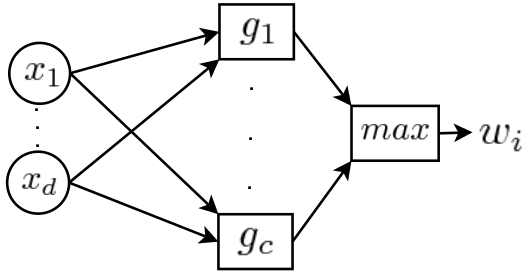
\includegraphics[width=0.3\textwidth-\fboxrule-\fboxrule]{clasificador.png}}  
\end{wrapfigure}	

\section{Bases estadísticas de reconocimiento de patrones}

\begin{description}
\item \textbf{Patrón.} Objeto de interés que es identificable del resto.
\item \textbf{Objetivo del RP:} Crear sistemas informáticos que imiten la percepción y razonamiento humano.
\item \textbf{Paradigma de trabajo funcional:}
\begin{enumerate}
\item \textit{Adquisición y preproceso de datos:} vector numérico que representa al patrón natural.
\item \textit{Extracción de características:} información \textit{relevante} para la clasificación. Dado un conjunto de patrones $n$-dimensionales, se busca un nuevo conjunto de representaciones $p$-dimensionales (con $p<n$). Tiene como propiedades deseables:
\begin{multicols}{3}
\subitem + Unicidad.
\subitem + Precisión.
\subitem + Continuidad.
\end{multicols}
\item \textit{Clasificación:} decisión sobre la clase.
\end{enumerate}
\item \textbf{Clasificador estadístico:} máquina formada por $c$ discriminantes: $g_i : E \rightarrow \mathbb{R}, \; 1 \leq i \leq c$, tal que dado un patrón $\mathbf{x} \in E$, se le asigna una clase $w_i$ si $g_i(\mathbf{x}) >g_j(\mathbf{x}) \forall j \neq i$.
\end{description}

\section{Perceptrón Multicapa}

La arquitectura del \textbf{Perceptrón Multicapa} (o PM) surge por corregir las limitaciones que las redes iniciales, \textit{Adaline} y \textit{Perceptron} tenían, sobre todo en cuanto a separabilidad de funciones no lineales.

\begin{wrapfigure}{r}{0.65\textwidth}
  \label{fig:layers}
  \caption{Interpretación geométrica del rol de las neuronas ocultas en un espacio de dos entradas.}
  \centering
  \hbox{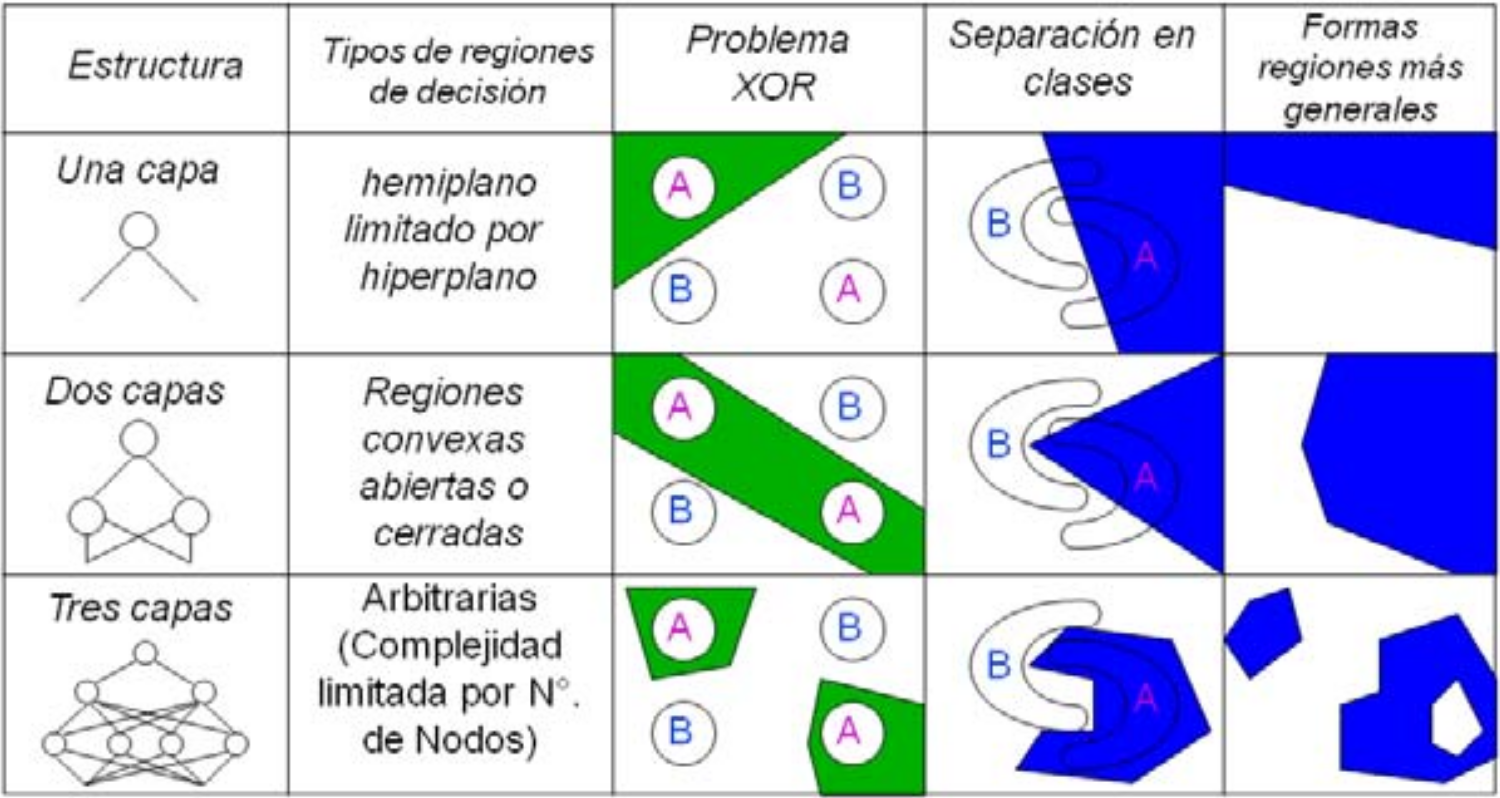
\includegraphics[width=0.65\textwidth-\fboxrule-\fboxrule]{layers.png}}  
\end{wrapfigure}	

Una de las ventajas de este tipo de red, entre otros, es que es un \textbf{aproximador universal de funciones}, de modo que cualquier función continua en el espacio multidimensional real se puede aproximar mediante una red PM.

Por otra, el PM es de relativo fácil uso y aplicación, dado que es una red sin recurrencias y \textit{feed-fordward}. Posee además una elevada capacidad de generalización y robustez, que provoca que la pérdida de una neurona no afecte al resultado.

La arquitectura del PM está basado en una red \textit{feed-fordward} o con conexiones hacia delante, en la que se disponen de 3 tipos de capas:
\begin{itemize}
\item La capa de \textbf{entrada}, en la que las neuronas actúan como buffer y no se disponen de pesos ni umbrales.
\item Las capas \textbf{ocultas}
\item La capa de \textbf{salida}, que actúa como un buffer de salida.
\end{itemize}

Todas las neuronas de la red (excepto las de la entrada, en general) llevan asociado un \textit{umbral}. Además, cada neurona de una capa tiene conexiones con todas las de la capa anterior, aunque puede suceder que en ciertos casos no sea así, y que el peso de una conexión sea 0, es decir, que no exista.

El entrenamiento de este tipo de redes, es decir, su aprendizaje, se realiza utilizando el \textbf{algoritmo de retropropagación}.

\subsection{Término de momento}
Si $\eta$ es chico, más chicos son los cambios en los pesos sinápticos, pero más lento es el aprendizaje. Si $\eta$ es grande, resulta en grandes cambios en los pesos sinápticos, pero puede provocar \textit{inestabilidad} (oscilaciones). Para solventar los problemas, agregamos una \textit{constante de momento}:
\[\Delta w_{ji}(n)=\alpha \Delta w_{ji}(n-1)+\eta \delta_j(n)y_i(n).\]

La inclusión del términomomento influye de la siguiente forma:

\begin{itemize}
\item Cuando $\partial \mathcal{E} (t) / \partial w_{ji}(t)$ tiene el mismo signo en sucesivas iteraciones: $\Delta w_{ji}(n)$ crece en magnitud y los $w_{ji}(n)$ se ajustan por un gran valor. El \textbf{momento} acelera la convergencia del método en direcciones largas de descenso.
\item Si $\partial \mathcal{E} (t) / \partial w_{ji}(t)$ tiene diferente signo en sucesivas iteraciones: el $\Delta w_{ji}(n)$ disminuye en magnitud y los $w_{ji}(n)$ se ajustan por un pequeño valor. El \textbf{momento} tiene un efecto \textit{estabilizante} en regiones oscilantes y ayuda a evitar a que se quede en un mínimo local.
\end{itemize}

\section{Red neuronal de Base Radial}

Modelo matemático:
\begin{align*}
&y_k (\mathbf{x}_l) = \sum_{j=1}^M w_{kj} \phi_j (\mathbf{x}_l), 
&&\text{con} \quad \phi_j (\mathbf{x}_l) = e^{-\frac{-||\mathbf{x}_l - \mathbf{\mu}_j||^2}{2 \sigma_j^2}}
\end{align*}
dónde $\mathbf{x}$ es el vector de entrada, $\mathbf{\mu}$ es el centroide, y $\sigma$ el factor suavizante o ancho.

\textit{Nota:} Los valores de $\sigma$ son encontrados una vez que ha terminado el \textit{clustering}. Como suelen ser medidos en base al \textit{spread} de cada nodo, normalmente se calculan como la distancia promedio de los patrones con cada centroide:
\[\sigma_j^2 = \frac{1}{M_j} \sum ||\mathbf{x} - \mathbf{w}_j||^2\]

\begin{wrapfigure}{r}{0.5\textwidth}
  \label{fig:radial}
  \caption{Arquitectura de una red neuronal de Base Radial.}
  \centering
  \hbox{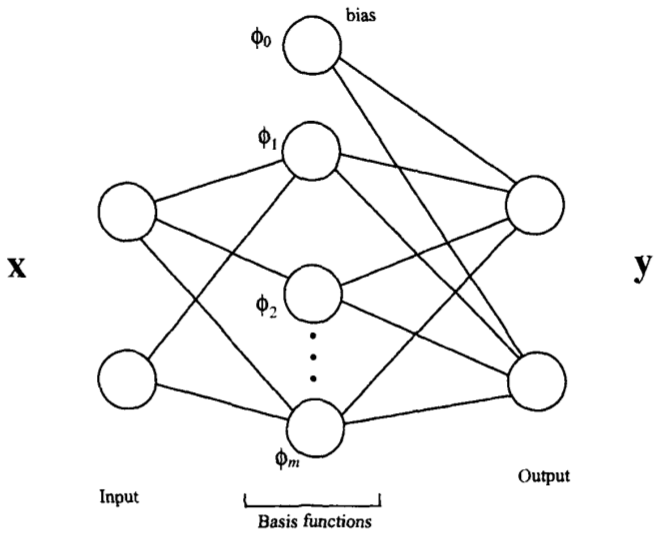
\includegraphics[width=0.5\textwidth-\fboxrule-\fboxrule]{radial.png}}  
\end{wrapfigure}	

\subsection{Adaptación de las RBF:\textit{k-means}}
Es un método NO supervisado, cuyo objetivos son:
\begin{enumerate}
\item Encontrar $k$ conjuntos $C_j$ de forma que:
\subitem + Cada conjunto $C_j$ sea lo más diferente posible de los demás.
\subitem + Los patrones $\mathbf{x}_l$ dentro de cada $C_j$ sean los más parecidos posibles entre ellos.
\item Encontrar el centroide $\mathbf{\mu_j}$ de cada conjunto $C_j$.
\end{enumerate}

\subsubsection{Algoritmo de adaptación \textit{batch k-means}:}
\begin{enumerate}
\item Inicialización: se forman los $k$ conjuntos $C_j(0)$ con patrones $\mathbf{x}_l$ elegidos aleatoriamente.
\item Se calculan los centroides:
\[\mathbf{\mu}_j(n) = \frac{1}{|C_j(n)}\sum_{l\in C_j(n)} \mathbf{x}_l\]
\item Se reasignan los $\mathbf{x}_l$ al $C_j$ más cercano:
\[ l \in C_j(n) \iff ||\mathbf{x}_l -\mathbf{\mu}_j||^2 < ||\mathbf{x}_l -\mathbf{\mu}_i||^2 \quad \forall i\neq j\]
\item Volver a 2 hasta que no se realicen reasignaciones.
\end{enumerate}

\subsubsection{Métodos de entrenamiento de pesos:}
\paragraph{Pseudo-inversa del vector $\phi(\mathbf{x}_l)$:} La solucion viene dada por la expresión: $W = G^{+} S$ (con $^+$ representando la pseudo-inversa, dada por $G^+=(G^T G)^{-1}G^T$), dónde $W$ es la matriz de orden $(n+1)\cdot r$ que posee los $n$ pesos y los umbrales en la última fila. La matriz G posee todas las funciones de activacion para cada uno de los patrones de entrada, es de orden $(n+1)\cdot N$, siendo $g_{in} = \phi_i(n)$ y $\phi_i$ la funcion de activacion de la neurona oculta $i$ para el patron de entrada $X(n)$. $S$ es la matriz de salidas deseadas de la red, de orden $N\cdot r$.

\paragraph{LMS:}
\begin{align*}
e_k(n) &= y_k(n)-d_k(n) ,\\
\mathcal{E} = \frac{1}{2} \sum_k e^2_k(n) &= \frac{1}{2} \sum_k \left(\sum_j w_{kj}(n)\phi_j(n)-d_k(n)\right)^2 ,\\
\frac{\partial \mathcal{E}(n)}{\partial w_{kj}(n)} &= (y_k(n) - d_k(n))\frac{\partial}{\partial w_{kj}} \left(\sum_j w_{kj} \phi_j(n) - d_k(n)\right), \\
\frac{\partial \mathcal{E}(n)}{\partial w_{kj}(n)} &= e_k(n) \phi_j(n)
\end{align*}
Regla de aprendizaje:
\begin{align*}
w_{kj}(n+1) &= w_{kj}(n) -\eta e_k(n) \phi_j(n) ,\\
w_{kj}(n+1) &= w_{kj}(n) -\eta \left(\sum_i w_{ki}(n) \phi_i(n) - d_k(n) \right) \phi_j(n)
\end{align*}

\subsection{Comparación entre las RBF y los MLP}

\begin{itemize}
\item Ambos son redes no-lineales de propagación hacia delante en capas.
\item Ambos son aproximadores universales.
\item Ambos pueden resolver el mismo tipo de problema.
\item Un RBF tiene sólo una capa oculta, mientras que el MLP puede tener una o más.
\item Las neuronas en las capas ocultas sirven a propósitos distintos en cada tipo de red.
\item En un RBF, la capa oculta es no lineal, mientras que la capa de salida es linear. En un MLP usado como clasificador de patrones, todas las capas son no lineales.
\item RBF usa la norma euclídea como argumento de la función de activación, mientras que el MLP usa el producto punto.
\item El RBF tiene representaciones locales sumadas, el MLP tiene representaciones distribuídas combinadas.
\item El RBF converge de forma más simple (\textit{lineal}), tiene un entrenamiento más rápido, arquitectura más simple, y una combinación de diferentes paradigmas de aprendizaje.
\end{itemize}

\section{Red de Hopfield}

La red de \textit{Hopfield} consiste en un grupo de neuronas y su correspondiente conjunto de unidades de retraso, formando un \textit{multiple-loop feedback system}. El número de búcles de retropropagación es igual al número de neuronas. Básicamente, la salida de cada neurona es retroalimentada, con un cierto desfasaje de una unidad, al resto de las neuronas de la red.

\subsection{Características}

Este tipo de red se \textbf{engloba} dentro de las redes totalmente recurrentes y se caracteriza porque cada una de las neuronas de la red tiene conexión con todas las demás.

\begin{wrapfigure}{r}{0.5\textwidth}
  \label{fig:hopfield}
  \caption{Arquitectura de una red de Hopfield.}
  \centering
  \hbox{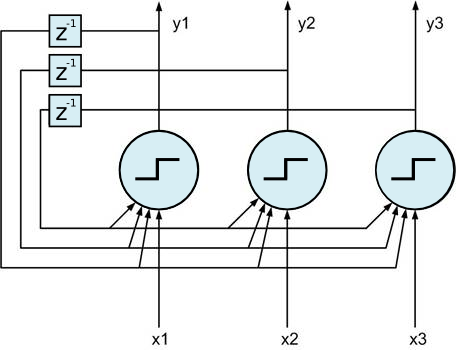
\includegraphics[width=0.5\textwidth-\fboxrule-\fboxrule]{hopfield.png}}  
\end{wrapfigure}	

El funcionamiento de la red es el de una \textbf{memoria asociativa}, permitiendo el almacenamiento y recuperación de patrones incluso cuando estos están incompletos. Los patrones que procesa son estáticos, aunque su procesamiento es temporal, es decir, la red requiere de un cierto tiempo de evolución hasta ofrecer la salida.

La filosofía de la red \textit{Hopfield} es diferente al de resto de redes. Su arquitectura carece de entradas o salidas en forma de neuronas. En el caso de estas redes, se habla del estado de la red. Es decir, se inicializan las neuronas a un cierto valor y la red evoluciona hacia un estado estable, que corresponderá con la salida asociada a la entrada.

Este tipo de arquitectura se utiliza mucho para optimización y reconstrucción de patrones a partir de datos incompletos.

\subsection{Fases de Operación}
\subsubsection{Fase de Almacenamiento}
Se determinan los valores que tendrán los pesos para almacenar un conjunto de patrones.
\begin{enumerate}
\item Conjunto de patrones que se desea almacenar: \{$\mathbf{x}(k)=(x_1(k), x_2(k), ..., x_n(k)$\}$_{k=1,...,p}$.
\item Aplicando aprendizaje Hebbiano:
\[w_{ji}=\frac{1}{N}\sum_{k=1}^p x_{j}(k) x_{i}(k)\]
\end{enumerate}

\subsubsection{Fase de Recuperación}
Mecanismo para recuperar la información almacenada a partir de
información incompleta.
\begin{enumerate}
\item Dado un patrón $\mathbf{x}$ (incompleto), se fuerza: $\mathbf{y}(0)=\mathbf{x}$;
\item $j^* = rand(N)$;
\item $y_{j^*}(n) = sign\left(\sum_{i=1}^N w_{ji} y_i (n-1)\right)$;
\item Volver a 2 hasta no observar cambios en $y_{j^*}$.
\end{enumerate}

\subsection{Generalidades}
\begin{multicols}{2}
\begin{itemize}
\item Cada neurona tiene un disparo probabilístico.
\item Conexiones simétricas.
\item El entrenamiento es no-supervisado.
\item Puede utilizarse como memoria asociativa.
\item Cada patron es un "valle" de energía.
\item Se busca el valle iterativamente a partir de ciertas condiciones iniciales.
\item El proceso de \textbf{entrenamiento} es NO iterativo.
\item El proceso de \textbf{recuperación} si ES iterativo (dinámico).
\item La capacidad de almacenamiento con un 1\% de error está limitada a: 
\[p_{max} = \frac{N}{2 ln(N)}.\]
\end{itemize}
\end{multicols}

\subsection{Redes Dinámicas de Elman y Jordan}

Las redes \textbf{Elman} y \textbf{Jordan} son redes parcialmente recurrentes, es decir, son redes con conexionado \textit{feed-fordward}, a las que se le han añadido algunas conexiones hacia atrás.

\begin{wrapfigure}{r}{0.45\textwidth}
  \label{fig:elman_jordan}
  \caption{Arquitectura de una red de Elman (\textit{arriba}) y una red Jordan (\textit{abajo}).}
  \centering
  \hbox{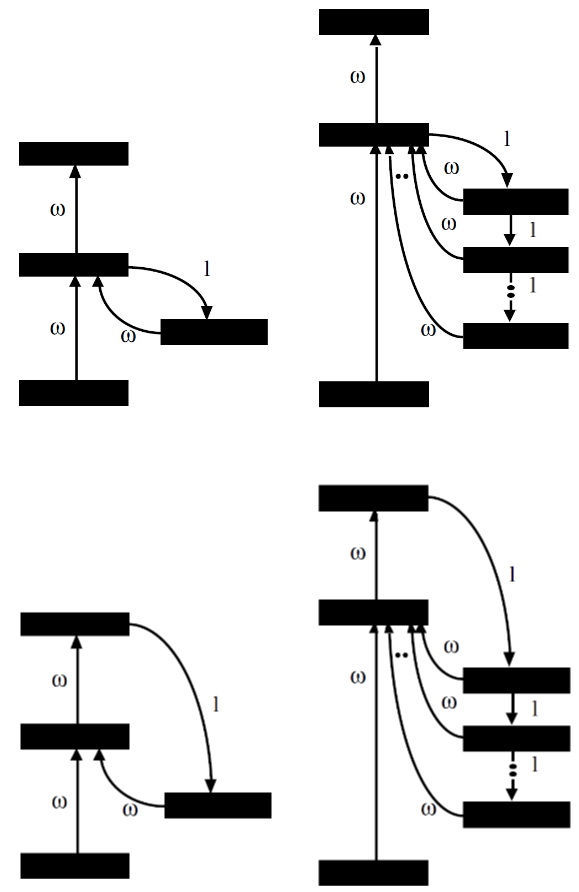
\includegraphics[width=0.45\textwidth-\fboxrule-\fboxrule]{elman_jordan.png}}  
\end{wrapfigure}	

Tanto en la red \textbf{Elman} como en la \textbf{Jordan}, la arquitectura básica de la red es básicamente una red \textit{feed-fordward}, y, en concreto, un PM, dado que las activaciones de todas las neuronas son saturantes. Sin embargo, de todas las entradas de las que se dispone en la capa de entrada algunas son utilizadas para recoger la información de la que disponían otras neuronas en el instante anterior. Estas neuronas se denominan \textbf{entradas de contexto}, dado que hacer referencia al estado anterior de la red.

La diferencia principal entre los dos tipos de arquitectura está en la información que se transmite a las entradas de contexto. En las redes \textbf{Elman}, se realimentan las salidas de las neuronas de la última capa oculta, de modo que, en cierto sentido, la red dispone de información acerca de la entrada del instante anterior.

En las redes \textbf{Jordan}, sin embargo, existe una doble recurrencia. Por una parte se realimentan las salidas del instante anterior ponderadas con un parámetro fijo $\mu$, y además, cada neurona de contexto recibe una copia de su estado anterior. El parámetro $\mu$ determina el horizonte de la memoria de la red, es decir, determina la ventana de tiempo que recuerda la red los datos de salida.

El aprendizaje de estos dos tipos de redes se basa en el algoritmo de retropropagación, dado que a la hora de entrenar se desacoplan los bucles. De este modo, inicialmente se calculan las salidas y se hallan los datos para pasar a las neuronas de contexto. En el siguiente instante, se consideran estos datos como entradas a la red, y se aplica de nuevo el algoritmo, y así sucesivamente.

\section{Redes Competitivas}

Las \textbf{redes competitivas} son muy utilizadas en la resolución de problemas de clasificación, aunque en algunos casos también se utilizan para la extracción de características relevantes, sobre todo aplicados a aprendizajes no supervisados.

En general, no suelen tener arquitecturas muy complejas, y en muchas ocasiones constan únicamente de dos capas: la \textbf{capa de entrada} y la llamada \textbf{capa de competición}, que todas ellas disponen.

En las \textit{capas de competición} las neuronas se conectan entre ellas en lo que se llama ''\textit{modelo de interacción lateral}''. Es decir, cada neurona de la capa competitiva se conecta con el resto, pero de diferente manera. Si la neurona se activa, intentará potenciar la activación de las neuronas de alrededor, incluyéndose a sí misma, y generará señales de deshabilitación a las neuronas que quedan lejos. El resultado del proceso es que sólo una neurona de entre todas queda activa, con su valor máximo. Es por ello por lo que se denomina a esta capa \textbf{competitiva}: las neuronas compiten entre ellas por la activación, y aquella que disponga de una señal más alta, porque sus pesos sean mayores, será la ganadora.

\subsection{Mapas Auto-Organizativos (SOM)}

Este tipo de red está basada en el aprendizaje \textit{competitivo}; las neuronas de salida de la red compiten entre ellas para ver cual será activada, dando como resultado que una sóla neurona, o neurona por grupo, es activada a la vez (\textit{winner takes all}).

Los SOM, además, como su nombre indica, se organizan sólos, es decir, como parte del aprendizaje, al activarse una neurona correspondiente a un ejemplo, la neurona evoluciona en el espacio, moviéndose hacia el punto del hiperespacio de entrada en el que está el ejemplo.

Este movimiento, sin embargo, no sólo afecta a la neurona activa, sino a las de su vecindario, es decir, las neuronas de alrededor, que son desplazadas ligeramente con esta, como si de una malla se tratara.

De este modo, las neuronas se irán desplazando por el espacio de entrada, hasta quedar agrupadas formando una malla en aquellas zonas del espacio de entrada a las que correspondan las entradas introducidas.

Por lo tanto, estos mapas nos permiten detectar relaciones entre los ejemplos y características comunes. También se utilizan para compresión y optimización de datos.

\subsubsection{Fases del proceso adaptativo (\textit{Haykin}, p452)}
\paragraph{Ordenamiento.} Ocurre el ordenamiento topológico de los pesos. Dura cerca de 1000 iteraciones, y a veces más.
\begin{itemize}
\item La $\eta$ debe comenzar con un valor cercano a 0.1; y luego decrecer gradualmente, pero permanecer por arriba de 0.01.
\item La función vecindad $h_{j,i}(n)$ debería incluir inicialmente toda las neuronas de la red, centrada en la neurona ganadora $i$, y luego achicarse con el tiempo.
\end{itemize}

\paragraph{Convergencia.} Ocurre el ajuste fino para asegurar una precisa cuantificación estadística. La cantidad de iteraciones es cercana a 500 veces el número de neuronas en la red.
\begin{itemize}
\item La $\eta$ debe mantenerse a un pequeño valor, del orden de 0.01. No debe reducirse nunca a cero, porque puede llevar a un estado \textit{metaestable}.
\item La función vecindad $h_{j,i}(n)$ debería incluir sólo las neuronas más cercanas, e incluso solamente a la neurona ganadora $i$.
\end{itemize}

\section{Lógica}
Las \textbf{lógicas} son \textbf{lenguajes formales} para representar información y o conocimiento de una forma que sea \textbf{tratable por computadoras}.
\begin{description}
\item \textbf{Sintaxis:} define cómo deben ser las oraciones en el lenguaje.
\item \textbf{Semántica:} define el significado de las oraciones (por ejemplo: define la veracidad de una oración)
\end{description}
La validez de los hechos o proposiciones puede probarse mediante \textbf{tablas de verdad} o a través de \textbf{Reglas de Inferencia}, las cuales se basan en la propiedad de \textbf{monotonicidad}.

\paragraph{Deducción o Inferencia.}
Relación entre un conjunto de proposiciones y una proposición tal que la última, denominada \underline{conclusión}, se obtiene necesariamente del primer conjunto, cuyos elementos se llaman \underline{premisas}.  Esta relación lógica cumple la propiedad de \textbf{monotonicidad}: las conclusiones se mantienen ante cualquier incremento de premisas.

\begin{quote}
Supongamos que una \textbf{Base de Conocimiento (BC)} justifica un conjunto de afirmaciones. Una lógica es \textbf{monótona} si cuando agregamos nuevas afirmaciones a la \textbf{BC}, todas las afirmaciones implicadas originalmente siguen siendo implicadas por la \textbf{BC} ampliada.
\[\text{Si }BC1 \: \models a \Rightarrow (BC1 \wedge BC2)\: \models a\]
\end{quote}

\subsection{Sistemas de producción con encadenamiento hacia adelante}
\begin{wrapfigure}{r}{0.4\textwidth}
  \label{fig:encadenamiento}
  \caption{Componentes de un Sistema de producción con encadenamiento hacia delante. M.I: \textit{Máquina de inferencia}; M.P: \textit{Memoria de producción}; M.T: \textit{Memoria de trabajo}.}
  \centering
  \hbox{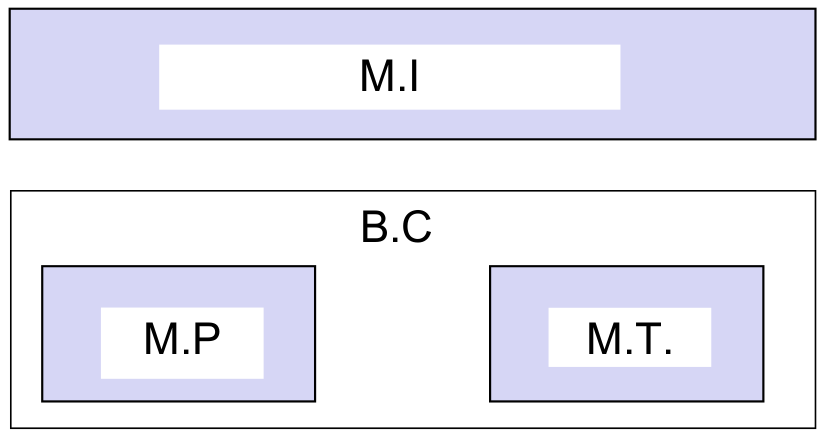
\includegraphics[width=0.4\textwidth-\fboxrule-\fboxrule]{encadenamiento.png}}  
\end{wrapfigure}
Se comienza desde las sentencias atómicas (hechos) de la memoria de trabajo y se infiere añadiendo las sentencias atómicas nuevas hasta que no se puedan realizar más inferencias o hasta que el objetivo haya sido agregado.

Cada inferencia es la aplicación de \textit{Modus Ponens}:
\[P \rightarrow Q, \; P \models Q\]

\subsubsection{Componentes:}
\begin{description}
\item \textbf{Memoria de Trabajo (MT):} Contiene un conjunto de literales positivas que no contienen variables (ej: \textit{perro tiene pelo}).
\item \textbf{Memoria de Producciones (MP):} está constituidas por reglas del tipo:
\begin{verbatim}
if <cond 1><cond 2>...<cond n> then <acc 1><acc 2>...<acc n>
\end{verbatim}
\subitem + \textit{Lado izquierdo} (antecedentes): puede contener variables, debe aparear con una afirmación.
\subitem + \textit{Lado derecho} (consecuentes): especifica acciones sobre la MT.
\end{description}

\subsubsection{Fases:}
\begin{enumerate}
\item \textbf{Match (fase de cotejo):} Se compara cada elemento de la premisa con el contenido de la MT. Se incorporan al \textbf{conjunto de conflicto} aquellas reglas cuya premisas se satisfacen con la MT actual.
\item \textbf{Resolución de conflictos:} Se decide cuál de las reglas contenidas en el \textbf{conjunto de conflicto} se va a ejecutar. Entre los criterios empleados se pueden mencionar: la más específica, la satisfecha con hechos más recientes, etc. 
\subitem \underline{\textit{Estrategias}}:
\subitem + No duplicación.
\subitem + Novedad.
\subitem + Específicidad.
\subitem + Prioridad de operación.
\item \textbf{Aplicación:} Se aplica el \textbf{consecuente} de la regla seleccionada. Se agregan a la MT los hechos que componen el \textbf{consecuente} o se ejecutan las acciones.
\end{enumerate}

\end{document}